\documentclass[conference]{assets/latex/IEEEtran}
\IEEEoverridecommandlockouts

\usepackage{amsmath,amssymb,amsfonts}
\usepackage{graphicx}
\usepackage{textcomp}
\usepackage{xcolor}

\graphicspath{{assets/latex/}}

\begin{document}

\title{CS6524 Computer Vision Lab. 4\\ Optical Flow and Kalman Filters}

\author{\IEEEauthorblockN{Darragh Luby}
\IEEEauthorblockA{\textit{University of Limerick} \\
ID 23359048}
\and
\IEEEauthorblockN{Aaron Roche}
\IEEEauthorblockA{\textit{University of Limerick} \\
ID 23359285}
\and
\IEEEauthorblockN{Ois\'{i}n Frizzell}
\IEEEauthorblockA{\textit{University of Limerick} \\
ID 23368276}
}

\maketitle

\begin{abstract}
We track a moving object with pyramidal Lucas--Kanade optical flow (OF), represent it by a single anchor point moved by the object's median flow, and fuse the measured position and velocity in a constant-velocity Kalman filter (KF) that bridges an artificial occlusion. Measuring velocity, not only position, cuts the error at reappearance in video~01 from 575 to 119\,px. The dominant remaining error is not the motion model but a measurement bias: near the occluder only part of the object is visible, so the measured position lags on entry and leads on exit by up to one object width. Feeding only velocity for the last 10 frames before the occlusion reduces the 01 error to 68\,px.
\end{abstract}

\section{Methodology}

\subsection{Optical flow and what we track}
Each frame pair is converted to greyscale. Corners are found with \texttt{goodFeaturesToTrack} (200 corners, quality 0.01, min.\ distance 5\,px), but only inside a mask of pixels whose absolute frame difference exceeds 15 grey levels, dilated by $15{\times}15$. Without the mask, the textured background and the checkerboard occluder take almost all corners. Points are followed with \texttt{calcOpticalFlowPyrLK} using a $21{\times}21$ window and \texttt{maxLevel}=3; four pyramid levels comfortably cover the fastest motion we see (${\approx}20$\,px/frame in 01 and 03). Points are carried over between frames instead of being re-detected; together with the grouping below, this halved the frame-to-frame position noise in 01 (robust $\sigma$ from 6.7/10.3\,px to 3.6/5.3\,px in $x$/$y$). A point is kept only if (i) the forward--backward error is below 1\,px, which removes points that slide along the occluder's edge, and (ii) it moved more than 1\,px.

Surviving points are grouped by drawing a 40\,px disc around each and taking connected components; groups with fewer than 5 points are discarded. Each group has a centroid $c$ and a velocity $v$, the medians of its points' positions and displacements. To acquire the object we take the fastest group within $45^\circ$ of the last known velocity, which rejects the hand that pushes the potato in 03.

\textbf{What we track: one anchor point.} Our first version used $c$ itself as the measured position. Because points keep joining and leaving the group (new corners every frame, points dropping under 1\,px/frame, the object splitting into 2--3 groups), $c$ jumped more than 15\,px away from $c_{t-1}+v_t$ in 49, 43 and 39 frames of 01, 02 and 03, and by up to 240\,px. We now track a single anchor $a$, initialised at $c$ and then moved by the flow and pulled slightly towards the centroid:
\begin{equation}
a_t = (a_{t-1}+v_t) + \alpha\,\bigl(c_t-(a_{t-1}+v_t)\bigr),\qquad \alpha=0.1 .
\end{equation}
While following, the group must lie within 150\,px of $a_{t-1}+v_{t-1}$ and within $45^\circ$ of $v_{t-1}$, and the nearest one is taken. After 3 frames without a group the anchor is dropped and re-acquired. The measurement is $z=[a_x,a_y,v_x,v_y]^\top$ in px and px/frame. No frame now deviates from the flow by more than 14\,px.

\subsection{Kalman filter design}
The state is $x=[p_x,p_y,v_x,v_y]^\top$ with $\Delta t=1$ frame and a constant-velocity transition
\begin{equation}
F=\begin{bmatrix} I_2 & I_2\\ 0 & I_2\end{bmatrix},\qquad H=I_4 .
\end{equation}
There is no control input, so $G$ is omitted. We measure velocity because OF gives it directly and it is far more precise than position: estimated from the data (below), $\sigma_v=0.06$--$0.54$\,px/frame against $\sigma_p=4$--$26$\,px.

\textbf{Measurement noise $R$.} For velocity, if measurements were exact then $v_t=v_{t-1}$; the residual over consecutive measured frames is a difference of two noisy measurements, so $\sigma_v=1.4826\,\mathrm{MAD}/\sqrt2$. For position this trick no longer works: the anchor is built from the flow, so $a_t-a_{t-1}-v_t$ is almost zero and gave $\sigma_p\approx0$, which made the filter treat the anchor as exact. Instead, $\sigma_p=1.4826\,\mathrm{MAD}(c_t-a_t)$, i.e.\ how far the anchor sits from the object's visible centroid. $R=\mathrm{diag}(\sigma_{p_x}^2,\sigma_{p_y}^2,\sigma_{v_x}^2,\sigma_{v_y}^2)$ is estimated separately for each video. MAD rather than standard deviation is used because single-frame glitches of ${\sim}100$\,px would otherwise inflate $R$ several times. With fewer than 10 consecutive pairs (our 04 video) we fall back to $\sigma_p=10$, $\sigma_v=0.5$.

\textbf{Process noise $Q$.} We use the discrete white-noise acceleration model, $Q=\sigma_a^2\,gg^\top\otimes I_2$ with $g=[\tfrac12,1]^\top$, so an unmodelled acceleration $a\sim\mathcal N(0,\sigma_a^2)$ moves position by $a/2$ and velocity by $a$ per frame. We chose $\sigma_a=0.1$\,px/frame$^2$ by sweeping 0.01--2 (Table~\ref{tab:err}); the reappearance error varied by less than the error itself, so we kept a value that lets the filter follow the slow decelerations in 01 without forgetting the velocity during a 70-frame occlusion.

\textbf{Initial state.} $x_0$ is the first measurement and $P_0=R$: the filter starts exactly as uncertain as that measurement.

\textbf{Gain.} After ${\sim}30$ frames, $K$ settles to ${\approx}0.03$--$0.05$ on the position-to-position terms but ${\approx}0.6$--$1.0$ from measured velocity to estimated position. The filter effectively dead-reckons on the OF velocity and uses the measured position as a weak anchor. We use \texttt{cv2.KalmanFilter} for the algebra but copy \texttt{statePre}/\texttt{errorCovPre} into the posterior after every predict; otherwise consecutive predict-only steps restart from the last corrected state and the track freezes behind the occluder.

\subsection{Occlusion, split trajectories and plots}
On frames without a measurement we only predict. The reappearance frame $r$ is the end of the longest gap. At $r$ we first record the prediction, which gives the error metric $e=\lVert \hat p_{r}^{-}-z_{p,r}\rVert$, then call \texttt{forecast} to roll $F$ forward from that state with no further corrections: the trajectory had the object not come back. In \texttt{XX\_tr.mp4} the corrected track is blue, the prediction-only track red, the counterfactual forecast pink, and white arrows show $5v$ every 10 frames.

\section{Results}

\begin{figure}[t]
\centerline{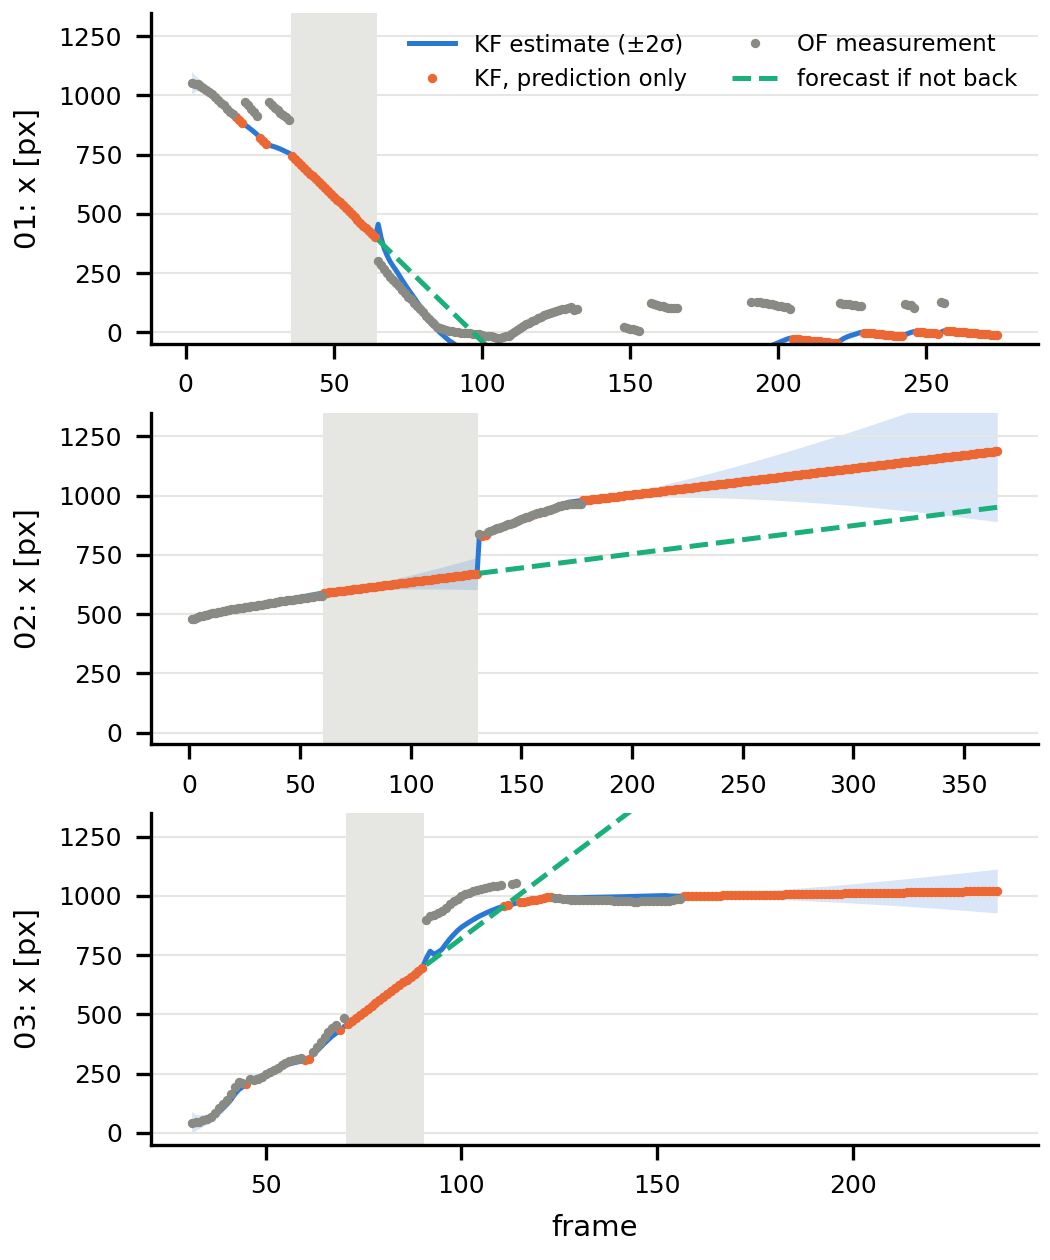
\includegraphics[width=\columnwidth]{fig_xt.png}}
\caption{Horizontal position over time. Grey: OF measurements; blue: KF estimate with $\pm2\sigma$ band; orange: prediction-only frames; green dashed: forecast if the object had not reappeared; shaded: main occlusion.}
\label{fig:xt}
\end{figure}

\begin{table}[t]
\caption{Error at reappearance $e$ [px] for the main occlusion}
\begin{center}
\begin{tabular}{lrrr}
\hline
 & 01 & 02 & 03 \\
\hline
Occluded frames & 29 & 70 & 20 \\
\textbf{Ours} (anchor, $H{=}I$, $\sigma_a{=}0.1$) & \textbf{119} & \textbf{303} & \textbf{208} \\
\quad filter $1\sigma_x$ at $r$ & 12 & 35 & 9 \\
Centroid $c$ as position (v1) & 262 & 290 & 112 \\
Position only ($H{=}[I_2\;0]$) & 575 & 361 & 280 \\
$\sigma_a=0.01$ & 163 & 261 & 259 \\
$\sigma_a=2$ & 149 & 320 & 175 \\
$\chi^2$ gate (99\%) & 652 & 248 & 684 \\
Velocity-only last 10 frames & 68 & 297 & 218 \\
\hline
\end{tabular}
\label{tab:err}
\end{center}
\end{table}

Fig.~\ref{fig:xt} and Table~\ref{tab:err} summarise the three provided videos. Reappearance errors are 119, 303 and 208\,px. Measuring velocity is the single most effective design choice: removing it from $H$ raises the error by 19--383\%, because the filter then has to infer velocity from position differences. $\sigma_a$ trades two failure modes: a small $\sigma_a$ holds the pre-occlusion speed (best in 02, where the speed changes behind the occluder) and a large one follows the latest measurements (best in 03). No single value wins all three. Fig.~\ref{fig:tracks} shows the overlays after reappearance.

\textbf{Anchor vs.\ centroid.} The anchor made the measured point stable in \texttt{XX\_of.mp4}, which was the goal, but it is not uniformly more accurate: the error fell from 262 to 119\,px in 01, while it rose from 290 to 303\,px in 02 and from 112 to 208\,px in 03. A pure flow-integrated anchor ($\alpha=0$) was worse still in 03: the hand's slower points share the potato's group, the median flow dropped to 2--6\,px/frame while the potato moved at ${\approx}12$, and the anchor fell 130\,px behind by frame 67. Sweeping $\alpha\in\{0,0.05,0.1,0.2,0.3\}$, $\alpha=0.1$ was the largest value that kept every step within 15\,px of the flow; at 0.2, 5--15 frames per video already exceed it.

\begin{figure}[t]
\centerline{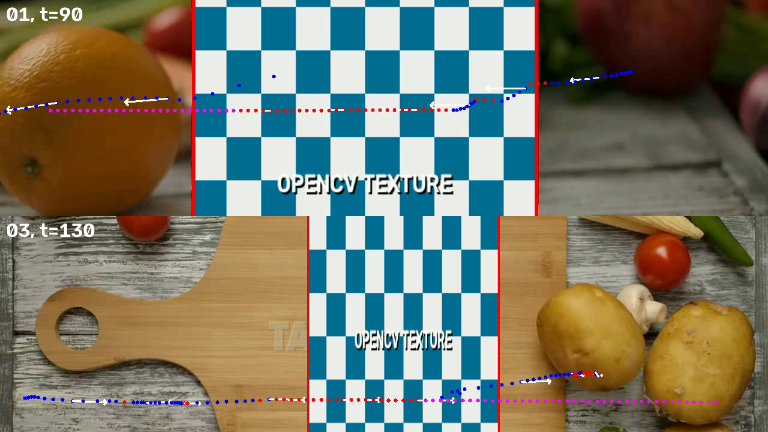
\includegraphics[width=\columnwidth]{fig_tracks.png}}
\caption{Output of \texttt{XX\_tr.mp4} after reappearance: blue measured/corrected, red predicted behind the occluder, pink counterfactual forecast, white velocity arrows.}
\label{fig:tracks}
\end{figure}

\section{Discussion and failure analysis}\label{sec:disc}

\textbf{Position bias at the occluder.} Fig.~\ref{fig:bias} shows 01 as the orange enters and leaves the occluder. At $t=30$ only the trailing sliver is visible, so the keypoints, and the anchor pulled towards them, lag the true centre; at $t=66$ the anchor is re-acquired on the only visible part, the leading edge. Between the last measurement before the gap and the first after it, the measured position moves 598\,px in 30 frames (19.9\,px/frame), while OF reports 12--15\,px/frame on both sides. Subtracting the orange's width (${\approx}250$\,px) gives 11.6\,px/frame, consistent with the flow. The velocity was right; the position was biased by up to one object width. With the centroid as position this bias produced the 262\,px error of v1; the anchor follows the flow into the occluder and halves it. Giving the filter only the velocity for the last 10 frames before the gap removes more of the entry bias and reduces the 01 error to 68\,px. It does not help 02 or 03, where other errors dominate.

\begin{figure}[t]
\centerline{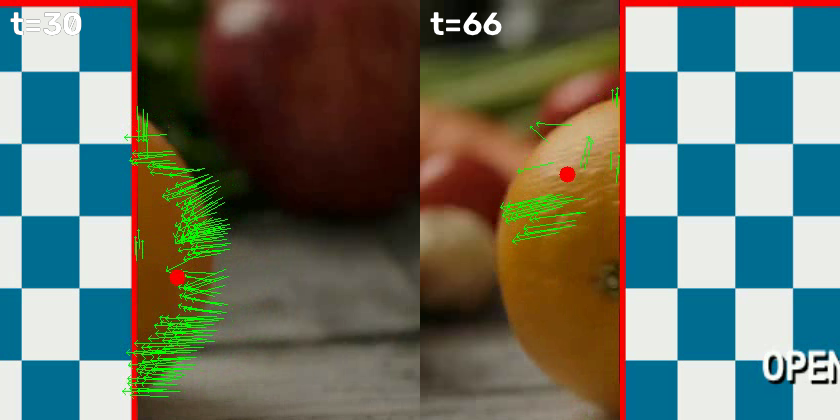
\includegraphics[width=\columnwidth]{fig_bias.png}}
\caption{\texttt{01\_of.mp4} entering ($t{=}30$) and leaving ($t{=}66$) the occluder. Green: LK flow ($3\times$); red: measured position (anchor), which can only follow the visible keypoints and so sits off the orange's true centre.}
\label{fig:bias}
\end{figure}

\textbf{Overconfident filter.} At reappearance the filter's own $1\sigma_x$ is 9--35\,px while the error is 119--303\,px. $R$ models zero-mean noise, but the occluder bias above is systematic and the same in every frame near the edge, so no diagonal $R$ represents it. It is also why a $\chi^2$ innovation gate, our first attempt at outlier rejection, failed: it rejected 26 and 33 valid measurements in 01 and 03, the filter drifted further, and errors rose to 652 and 684\,px (Table~\ref{tab:err}).

\textbf{Speed change during occlusion (02).} The pen moves at ${\approx}1.8$\,px/frame before and ${\approx}3.5$\,px/frame after the occlusion. No constant-velocity model can predict this; the 303\,px error is mostly the extra distance. The pen is also long and diagonal, so the visible part, and with it $p_y$, changes as it passes the occluder (430$\to$210\,px).

\textbf{Objects that stop.} Only points moving more than 1\,px/frame are kept, so the measured speed can never be much below 1\,px/frame and a stationary object gives either no measurement or a small false velocity. The filter keeps integrating it, and $K\approx0.04$ on position is too weak to pull it back. In 01, while the orange rests at $x\approx100$--$130$, the estimate drifts to $x\approx-11$ (off-screen), a median offset of 153\,px from the measurements after reappearance. In 02 the pen stops at $x\approx963$ (frame 177) while the filter reaches $x=1188$ by the last frame. Fixing $\sigma_p=5$\,px cuts the 01 offset to 53\,px but raises its reappearance error from 119 to 233\,px, so we kept the data-driven $R$.

\textbf{Bonus video (04).} Our own recording is 1080p and the object moves fast. Only 1 of 84 frames yields a measurement: the first, noisy velocity seeds the $45^\circ$ direction filter, which then rejects every later group. The video and its output are included, but the tracking does not work on it.
% TODO(team): update this paragraph if 04 is re-recorded or the OF settings are adapted.

\textbf{Improvements.} (1) Detect contact with the occluder mask and switch to a velocity-only measurement ($H=[0\;I_2]$) on entry, and on exit until the full group is visible. (2) Measure a size-aware centre, e.g.\ the leading edge plus half the object width estimated while fully visible. (3) Compute the velocity from all points of the followed group, including those under 1\,px/frame, so a stopped object reads $v\approx0$, and add a stopped mode (e.g.\ an IMM with constant-velocity and stationary models). (4) Exclude the hand from the potato's group in 03 (e.g.\ by colour), so the anchor's flow is not slowed. (5) Tune $R$ online from the normalised innovation squared.


\end{document}
